\documentclass[a4paper]{article}

\usepackage[T1]{fontenc}
%\usepackage[utf8]{inputenc}
%\usepackage[italian]{babel}
\usepackage{amssymb}
\usepackage{hyperref}
\usepackage{mathtools}
\usepackage{amsthm}
%\usepackage[ruled,vlined,noend]{algorithm2e}

%%%%%%%%%%%%%%%%%%%%%%%%%%%%%%%%%%%%
\usepackage{listings} 
\lstdefinestyle{mystyle}{
    breakatwhitespace=false,                   
    captionpos=b,                    
    keepspaces=true,                 
    numbers=left,                    
    numbersep=5pt,                  
    showspaces=false,                
    showstringspaces=false,
    showtabs=False,                  
    tabsize=2
}

\lstset{style=mystyle}

\usepackage{setspace}
\singlespacing
%%%%%%%%%%%%%%%%%%%%%%%%%%%%%%%%%%%%
\usepackage{ulem} 
\usepackage{soul}

\usepackage{graphicx}
\graphicspath{ {./images/} }
%%%%%%%%%%%%%%%%%%%%%%%%%%%%%%%%%%%%
\mathtoolsset{showonlyrefs}  
\hypersetup{
    colorlinks=true,
    linkcolor=black,
    filecolor=black,      
    urlcolor=black,
}

\newcommand{\pluseq}{\mathrel{{+}{=}}}

\newtheorem {theorem}{Theorem}
\newtheorem{corollary}{Corollary}
\newtheorem{lemma}{Lemma}
\newtheorem{remark}{Remark}
\newtheorem{definition}{Definition}

\setcounter{secnumdepth}{3}
\setcounter{tocdepth}{3}

\title{Advanced Programming}
\author{Federico Bruzzone}
%\date{}
\makeindex

\begin{document}
\maketitle
\newpage
% \setlength{\parskip}{0.15em}
\tableofcontents
\setlength{\parindent}{0pt}
\setlength{\parskip}{0.8em}
\newpage

%\section{section}
...

\subsection{subsection}
	
\paragraph{paragraph}

\begin{remark}
    ...
\end{remark}

\subsubsection{subsubsection}

\subsubsection{subsubsection}

\paragraph{paragraph}

\subsection{subsection}
...
\begin{enumerate}
    \item 
    \item
    \item 
\end{enumerate}

\begin{itemize}
	\item 
    \item 
\end{itemize}

\begin{theorem}
    $PO \subseteq NPO$
\end{theorem}
\begin{proof}
    ...
\end{proof}

\begin{equation}
    \begin{aligned}
        \mathit{APX} = \{\Pi | \Pi \mathit{\;di\;ottimizzazione\;t.c.\;}
\exists \rho \geq 1, A, \\\mathit{t.c\;} x\rightarrow A \rightarrow y(x)\;\mathit{con}\;R_\Pi(x, y) \leq \rho\}
    \end{aligned}
\end{equation}


\paragraph{Algoritmo di risoluzione}
L'algoritmo di risoluzione è abbastanza semplice e si basa sulla 
ricerca di un cammino aumentante.

\begin{algorithm}[H]
    \SetAlgoLined
    \KwIn{$G=(V,E)$}
    \KwResult{Matching $M$ per $G$}
     $M \gets \emptyset$\\
     \While{$\Pi = \mathit{findAugmenting(G)}$}{
        $M.update(\Pi)$
     }
     \Return{M}
     \caption{BiMaxMatching}
\end{algorithm}


\subsection{Tecniche greedy}
Nella sezione a seguire si presentano problemi di ottimizzazione per cui 
tecniche greedy funzionano abbastanza bene. 
I problemi affrontati sono quelli di \emph{Load Balancing}, \emph{Center Selection} e \emph{Set Cover}.

\subsubsection{Load balancing}
\label{lb}
Il problema di Load Balancing può essere visto come il compito
di assegnare a macchine dei lavori da compiere, che richiedono del tempo, 
in modo da minimizzare il tempo totale.


\begin{theorem}
    Load Balancing è NPO completo
\end{theorem}
Bisogna perciò trovare un modo di approssimare una soluzione.
\paragraph{Greedy balance}
Il primo approccio alla risoluzione del problema è quello di assegnare la prossima
task alla macchina più scarica in questo momento.

\begin{algorithm}[H]
    \SetAlgoLined
    \KwIn{$M$ numero di macchine, $t_0, \dots, t_n$ task}
    \KwResult{Assegnamento delle task alle macchine}
     $L_i \gets 0\;\forall i \in M$\\
     $\alpha \gets \emptyset$\\
     \For{$j = 0, \dots, n$}{
         $\hat{i} = \min(L_i)$\\
         $\alpha(j) = \hat{i}$\\
         $L_{\hat{i}} \pluseq t_j$
     }
     \Return{$\alpha$}
     \caption{GreedyBalance}
\end{algorithm}

\begin{lstlisting} %[language=Python, caption=Python example]

import numpy as np
    
def incmatrix(genl1,genl2):
    m = len(genl1)
    n = len(genl2)
    M = None #to become the incidence matrix
    VT = np.zeros((n*m,1), int)  #dummy variable
    
    #compute the bitwise xor matrix
    M1 = bitxormatrix(genl1)
    M2 = np.triu(bitxormatrix(genl2),1) 

    for i in range(m-1):
        for j in range(i+1, m):
            [r,c] = np.where(M2 == M1[i,j])
            for k in range(len(r)):
                VT[(i)*n + r[k]] = 1;
                VT[(i)*n + c[k]] = 1;
                VT[(j)*n + r[k]] = 1;
                VT[(j)*n + c[k]] = 1;
                
                if M is None:
                    M = np.copy(VT)
                else:
                    M = np.concatenate((M, VT), 1)
                
                VT = np.zeros((n*m,1), int)
    
    return M
\end{lstlisting}

%%%%%%%%%%%%%%%%%
\usepackage{listings}
\usepackage{xcolor}

\definecolor{codegreen}{rgb}{0,0.6,0}
\definecolor{codegray}{rgb}{0.5,0.5,0.5}
\definecolor{codepurple}{rgb}{0.58,0,0.82}
\definecolor{backcolour}{rgb}{0.95,0.95,0.92}

\lstdefinestyle{mystyle}{
    backgroundcolor=\color{backcolour},   
    commentstyle=\color{codegreen},
    keywordstyle=\color{magenta},
    numberstyle=\tiny\color{codegray},
    stringstyle=\color{codepurple},
    basicstyle=\ttfamily\footnotesize,
    breakatwhitespace=false,         
    breaklines=true,                 
    captionpos=b,                    
    keepspaces=true,                 
    numbers=left,                    
    numbersep=5pt,                  
    showspaces=false,                
    showstringspaces=false,
    showtabs=false,                  
    tabsize=2
}

\lstset{style=mystyle}
\section{}

\subsection{Informazioni generali}

\textbf{Scopo del corso}
\begin{itemize}
	\item Scoprire il concetto di separazione dei compiti;
	\item Imparare a programmare decomponendo le funzionalità del SW;
	\item Imparare ad ottimizzare il SW separandone le funzionalità;
	\end{itemize}
\textbf{Materiale di riferimento}
\begin{itemize}
	\item i licidi del corso;
	\item Ira R. Forman and Note B. Forman. Java Reflection in Action Manning Publications, October 2004;
	\item Ramnivas Laddad. AspectJ in Action: Pratical Aspect-Oriented Programming. Manning Pubblications Company, 2003;
\end{itemize}



















\subsubsection{How to use Python}	
\textbf{We are condidering Python 3+}
\begin{itemize}
	\item version > 3 is incompatible with previus version;
	\item version 2.7 is the current version.
\end{itemize}
\textbf{A python program can be:}
\begin{itemize}
	\item edited in the python shell and executed step-by-step by the shell;
	\item edited and run through the iterpreter.
\end{itemize}

\subsection{Overview of the Basic Concepts}	

\subsubsection{Our first Python program}
\hrule
\begin{lstlisting}[language=Python, caption=humanize.py]
SUFFIXES = {1000: ['KB', 'MB', 'GB', 'TB', 'PB', 'EB', 'ZB', 'YB'], 
            1024: ['KiB', 'MiB', 'GiB', 'TiB', 'PiB', 'EiB', 'ZiB', 'YiB']}
def approximate_size(size, a_kilobyte_is_1024_bytes=True):
	''' Convert a file size to human-readable form. '''
	if size < 0:
		raise ValueError('number must be non-negative')
	multiple = 1024 if a_kilobyte_is_1024_bytes else 1000
	for suffix in SUFFIX[multiple]:
		size /= multiple
		if size < multiple:
			return '{0:.1f} {1}'.format(size, suffix)
		raise ValueError('number too large')
				
if __name__ == '__main__':
	print(approximate_size(1000000000000, False))
	print(approximate_size(1000000000000))
\end{lstlisting}
\hrule	

\subsubsection{Declaring function}	
\textbf{Python has function}
\begin{itemize}
	\item no header files à la C/C++;
	\item no interface/implementation à la Java.
\end{itemize}			
\hrule
\begin{lstlisting}[language=Python]
def approximate_size(size, a_kilobyte_is_1024_bytes=True):
\end{lstlisting}	
\begin{enumerate}
	\item \textbf{def}: function definition keyword;
	\item \textbf{approximate\_size}: function name;
	\item \textbf{a\_kilobyte\_is\_1024\_bytes}: comma separate argument list;
	\item \textbf{=True}: default value.
\end{enumerate}
\hrule		
\textbf{Python has function}
\begin{itemize}
	\item no return type, it always return a value (\textbf{None} as a default); 
	\item no parameter types, the interpreter figures out the parameter type.
\end{itemize}	

\subsubsection{Calling Functions}
\textbf{Look at the bottom of the \textit{humanize.py} program}
\hrule
\begin{lstlisting}[language=Python]
if __name__ == '__main__':
	print(approximate_size(1000000000000, False))
	print(approximate_size(1000000000000))
\end{lstlisting}
\begin{enumerate}
	\item[2] in this call to \textbf{approximate\_size()}, the \textbf{a\_kilobyte\_is\_1024\_bytes} parameter will be \textbf{False} since you explicitly pass it to the function;
	\item[3] in this row we call  \textbf{approximate\_size()} with only a value, the parameter \textbf{a\_kilobyte\_is\_1024\_bytes} will be \textbf{True} as defined in the function declaration.
\end{enumerate}
\hrule
\textbf{Value can be passed by name as in}:
\hrule
\begin{lstlisting}[language=Python]
def approximate_size(a_kilobyte_is_1024_bytes=True, size=1000000000000)
\end{lstlisting}	
\hrule
\textbf{Parameters' order is not relevant}

\subsubsection{Writing readable code}
\textbf{Documentation Strings}
A python function can be documented by a documentation string (docstring for short).
\begin{center}
	\textit{''' Convert a file size to human-readable form.  '''}
\end{center}
\textbf{Triple quotes delimit a single multi-string}
\begin{itemize}
	\item if it immediatly follows the function's declaration it is the doc-string associated to the function;
	\item docstrings can be retrieved at run-time (they are attributes).
\end{itemize}
\textbf{Case-Sensitive}
All names in Python are case-sensitive

\subsubsection{Everything is an object}
\textbf{Everything in Python is an object, functions included}
\begin{itemize}
	\item \textbf{import} can be used to load python programs in the system as modules;
	\item the dot-notation gives access to the the public functionality of the imported modules;
	\item the dot-notation can be used to access the attributes (e.g., the \textbf{\_\_doc\_\_})
	\item \textbf{humanize\.approximate\_size.\_\_doc\_\_} gives access to the docstring of the \textbf{approximate\_size()} function; the docstring is stored as an attribute.
\end{itemize}

\subsubsection{Everything is an object (Cont'd)}
\textbf{In python is an object, better, is a \textbf{first-calss object}}
\begin{itemize}
	\item everything can be assigned to a variable or passed as an argument
\end{itemize}
\hrule
\begin{lstlisting}[language=Python]
h1 = humanize.approximate_size(9128)
h2 = humanize.approximate_size
\end{lstlisting}	
\begin{itemize}
	\item \textbf{h1} contains the string calculated by \textbf{approximate\_size(9128};
	\item \textbf{h2} contains the "function" object \textbf{approximate\_size()}, the result is not calculated yet;
	\item to simplify the concept: \textbf{h2} can be considered as a new name of (alias to) \textbf{approximate\_size}.
\end{itemize}
\hrule

\subsubsection{Indenting code}
\textbf{No explicit block delimiters}
\begin{itemize}
	\item the only delimiter is a column (':') and the code indentation;
	\item code blocks (e.g., functions, if statements, loops, ...) are defined by their indentation;
	\item white spaces and tabs are relevant: use them consistently;
	\item indentation is checked by the compiler.
\end{itemize}

\subsubsection{Exceptions}
\textbf{Exceptions are Anomaly Situations}
\begin{itemize}
	\item C encourages the use of return codes which you check;
	\item Python encourages the use of exceptions which you handles.
\end{itemize}
\textbf{Raising Exceptions}
\begin{itemize}
	\item the \textbf{raise} statement is used to rise an exception as in:
\begin{lstlisting}[language=Python]
raise ValueError('number must be non-negative')
\end{lstlisting}
	\item syntax recalls function calls: \textbf{raise} statement followed by an exception name with an optional argument;
	\item exceptions are relized by classes.
\end{itemize}
\textbf{No need to list the exceptions in the function declaration handling Exceptions}
\begin{itemize}
	\item an exception is handled by a \textbf{try} ... \textbf{except} block.
\hrule
\begin{lstlisting}[language=Python]
try:
	from lxml import etree
except ImportError:
	import xml.etree.ElementTree as etree
\end{lstlisting}
\hrule
\end{itemize}

\subsubsection{Running scripts}
\textbf{Look again, at the bottom of the \textit{humanize.py} program}:
\hrule
\begin{lstlisting}
if __name__ == '__main__':
	print(approximate_size(1000000000000, False))
	print(approximate_size(1000000000000))
\end{lstlisting}
\hrule
\textbf{Modules are Objects}
\begin{itemize}
	\item they have a built-in attribute \textbf{\_\_name\_\_}
\end{itemize}
\textbf{The value of \textbf{\_\_name\_\_} depends on how you call it}
\begin{itemize}
	\item if imported it contains the name of the file without path and extension.
\end{itemize}

\section{Computational Reflection}

\subsection{Computational Reflection}

\subsubsection{A first definition}

Computational reflection can be intuitively defined as:

\textit{"The activity done by a SW system to represent and manipulate its own structure and behavior"}

The reflective activity is done analogously to the usual system activity

\subsection{Reflection}

\subsubsection{Historical Overview}

\textbf{In the sisties}
\begin{itemize}
	\item Research field: artificial intelligence;
	\item First approaches to relection: intelligent behavior;
\end{itemize}

\textbf{In the eighties}
\begin{itemize}
	\item Research filed: programming languages;
	\item Brian C. Smith, he introduces the reflection in Lisp (1982 and 1984), the reflective tower has been defined;
	\item Several reflective list-oriented languages have been defined (they exploit the quoting machanism);
\end{itemize}

\textbf{In the meanwhile}
\begin{itemize}
	\item Research field: logic programming;
	\item the meta-programming takes place in PROLOG;
\end{itemize}

\textbf{Between the eighties and the nineties}
\begin{itemize}
	\item Research fild: object-oriented programming languages;
	\item Pattie maes defines the computational reflection in OOPL (1987);
	\item Several people move from Lisp to OO:
		\begin{itemize}
			\item P. Coite, ObjVLips (1987)
			\item A. Yonezawa, ABCL-R (1988)
			\item J. des Rivières e G. Kiczales MOP for CLOS (1991)
		\end{itemize}
	\item SmallTalk is elected as the best reflective programming language
\end{itemize}

\textbf{In te nineties}
\begin{itemize}
	\item Research field: typed and/or compiled object-oriented programming languages;
	\item Shigeru Chiba realizes OpenC++ (1993-1995), OpenJava (1999);
\end{itemize}

\textbf{In the 1997}
\begin{itemize}
	\item Gregor Kiczales et al. defined the aspect-oriented programming and the story ends;
\end{itemize}

\subsection{Computational Reflection}

\subsubsection{Reflection à la Pattie Maes}

\textbf{Pattie Maes has pioneered the filed}
\begin{itemize}
	\item a \textbf{computational system} is a system that can reason about and act on its applicative somain;
	\item a computational system is \textbf{causally connected} to its domain if and only if a change to its domain is reflected on it and vice versa;
	\item a \textbf{meta-system} is a computational system whose applicative domain in another computational system;
	\item \textbf{reflection} is the property of reasoning about and acting on itself;
\end{itemize}

\textbf{therefore}
\begin{itemize}
	\item a \textbf{reflective system} is a meta system causally connected to itself;
\end{itemize}

\subsubsection{Reflective system}

\textbf{From the definition, we can evince that a reflective system is:}
\begin{itemize}
	\item a software system logically layered into two or more levels respectively called base-level and meta-levels;
	\item the system running in a meta-level observes and manipulates the system running in the underlying level (reflective tower);
\end{itemize}

\textbf{Characteristics}
\begin{itemize}
	\item the system running in the base-level is unaware of the existence and of the work of the systems running in the overlying levels;
	\item a meta-level system acts on a representation (called the system running in the underlying levels; and
	\item a system and its reification are causally connected and therefore, they are kept mutually consistent
\end{itemize}

\subsubsection{Reflective system: Base- and Meta-levels}

\textbf{A meta-level system refies what it is implicit (e.g. mechanisms and structure) of the underlying base- or meta-level}

\subsubsection{How to Characterize a Reflective System}

\textbf{The reflective systems can be classified based on:}
\begin{itemize}
	\item what and when
\end{itemize}

\textbf{What kind of reflective actions the system can carry out:}
\begin{itemize}
	\item structural and behavioral reflection;
	\item introspection (just to observe) and intercession (to alter)
\end{itemize}

\textbf{When the meta-level entities exist:}
\begin{itemize}
	\item compile-time
	\item load-time; and
	\item run-time
\end{itemize}

\subsubsection{Behavioral and structural reflection}

\textbf{The behavioral reflection allows the program of monitoring and manipulating its own computation, e.g.:}
\begin{itemize}
	\item to trap a method call and activating a different method instead;
	\item to monitor the object state;
	\item to create new objects, and so on
\end{itemize}

\textbf{These activities can take place at run-time without a specific support}

\textbf{The structural reflection allows the program of inspecting and altering its own structure, e.g.:}
\begin{itemize}
	\item the code of a method can be modified or removed from the class;
	\item new methods and field can be added to a class, and so on;
\end{itemize}

\textbf{These activities need a specific support by the execution environment (from the VM, RTE, ...) to be carried out at run-time}

\subsubsection{Reification}
\textbf{The base-level entities (referents) are reified into the metalevel, i.e., they have a representative into the meta-level}

\textbf{Such a representative, called reification, has to:}
\begin{itemize}
	\item support all the operations and have the same characteristics of the corresponding referent;
	\item be kept consistent to its referent ( causal connection);
	\item be subjected to the manipulations of the meta-level entities to protect the base-level entities from potential inconsistency
\end{itemize}

\textbf{Any change carried out on the reification has to be reflected on the corresponding referent.}

\subsection{To Develop a Reflective System}
\textbf{Jacques Ferber [2] has raised some issues that the developers must take in consideration:}
\begin{itemize}
	\item which kind of entities should be reified?
	\item what and how it is implemented the causal connection?
	\item when does the execution shift to the meta-level?
\end{itemize}

\subsection{Which Kind of Entities Should Be Reified?}
\textbf{It depends on the programming language:}
\begin{itemize}
	\item functional: lambda expression/closures, environment, continuations, and so on ...;
	\item object-oriented: objects, methods, classes, messages and so on ...;
	\item concurrent and object-oriented: threads, processes, schedulers, monitors, and so on ...;
	\item distribution: namespaces, proxies, mailers, and so on ...
\end{itemize}

\subsection{What and How It Is Implemented the Causal Connection?}
\textbf{It depends on when the reflective activities take place:}
\begin{itemize}
	\item atrun-time: the causal connection is explicit and must be maintained by an entities super-parties, e.g., by the virtual machine or by the run-time environment;
	\item at compile-time: the causal connection is implicit, base-level and meta-levels are merged together during a preprocessing phase;
	\item at load-time: in this case the causal connection behaves as in the case, reflection takes place at compile-time;
\end{itemize}

\textbf{Most of the times, the supported reflective activity is related to observe (introspection) the base-level system so the causal connection become unilateral and can be managed by the metaentities.}

\subsection{When Does the Execution Shift to the Meta-Level?}
\textbf{Switching among levels depends on:}
\begin{itemize}
	\item which entities are reified;
	\item when such entities are reified; and
	\item how the causal connection is managed
\end{itemize}

\textbf{The shift-up and-down actions}
\begin{itemize}
	\item the shift-up and-down actions.
\end{itemize}

\textbf{When}
\begin{itemize}
	\item an observed element changes; or
	\item an action is going to be done;
\end{itemize}

\textbf{the computational flow passes into the meta-level (shift-up)}

\textbf{Instead}
\begin{itemize}
	\item the computational flow goes back (shift-down) on the meta-level program decision
\end{itemize}

\textbf{Usually, the shift-up action is managed by call-backs}

\section{Reflection in OO Programming Languages}

\subsection{Structural and Behavioral Reflection}

\textbf{Structural Reflection}
\begin{itemize}
	\item Object creation and init
		\begin{itemize}
			\item constructor
			\item prototype
			\item meta-classes
		\end{itemize}
	\item Class manipulation
		\begin{itemize}
			\item to add or remove fields
			\item to add or remove methods
			\item to change the super class
		\end{itemize}
\end{itemize}

\textbf{Behavioral Reflection}
\begin{itemize}
	\item message sending
		\begin{itemize}
			\item classes and inheritance
			\item prototypes and delegation
			\item errors
			\item encapsulations
			\item proxies
			\item meta-objects
		\end{itemize}
\end{itemize}

\subsection{Structural Reflection}
The objects running in the meta-level, called \textbf{meta-objects} are associated to all (or just to some of) the objects running in the base-level, called \textbf{referents}.

The connection among referents and meta-objects is called \textbf{causal connection} when it is a two-way link or \textbf{meta-connection} when it is a one-way link.

The meta-objects exist at run-time and extend or modify the semantics of some mechanisms:

-  method invocation, field access, object creation, and so on

The \textbf{MOP} is the set of messages that a meta-object can understand

\subsubsection{Es.To Enrich the Behavior of a Method Call}

\begin{center}
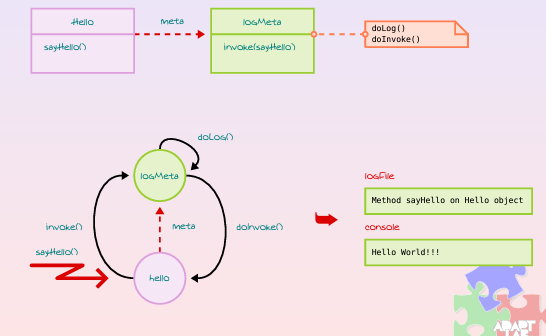
\includegraphics[scale=0.7]{1-To-Enrich-the-Behavior-of-a-Method-Call}
\end{center}

\subsubsection{Different views}

\begin{center}
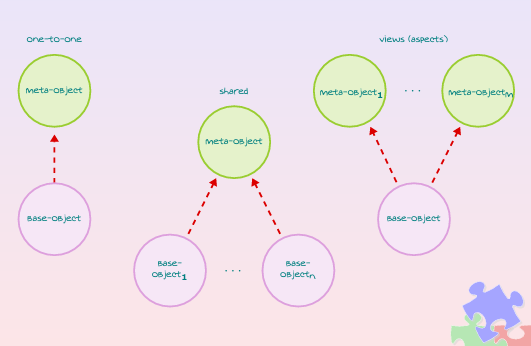
\includegraphics[scale=0.7]{2-different-views}
\end{center}

\subsubsection{Classes as meta objects}

\begin{center}
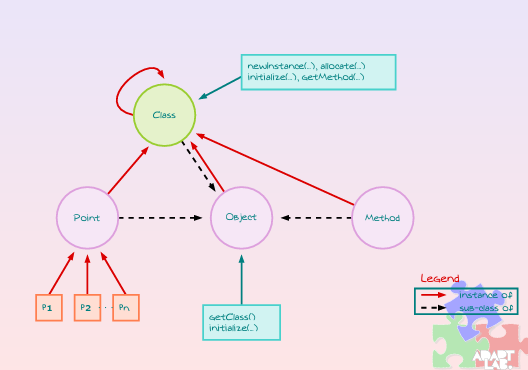
\includegraphics[scale=0.7]{3-classes-as-meta-objects}
\end{center}

\subsubsection{Classes AS Meta-Objects (Cont'd)}
\textbf{The meta-class based approach}
\begin{itemize}
	\item the classes carry out there flective activity
	\item the reflective tower is realized by the inheritance link
\end{itemize}

\textbf{Drawbacks}
\begin{itemize}
	\item all the instances of a classs hare the same meta-class therefore the same reflective behavior (the granularity of reflection is at the class level)
	\item the classes have to be available a trun-time
\end{itemize}

\textbf{Programming Languages}
\begin{itemize}
	\item SmallTalk (Adele Goldberg,1972)
	\item ObjVLisp (PierreCointe,1987)
	\item IBMSystemObjectModel (IBM,1992)
\end{itemize}

\subsubsection{Classes AND meta objects}

\begin{center}
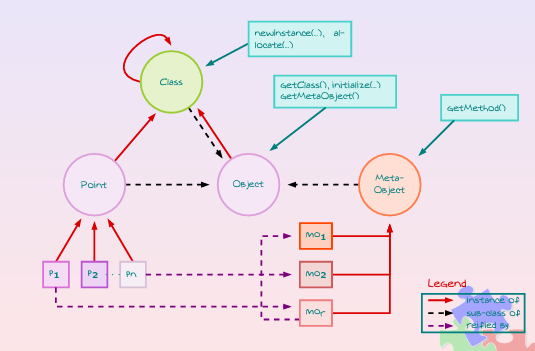
\includegraphics[scale=0.7]{4-classes-and-meta-objects}
\end{center}

\subsubsection{Classes AND Meta-Objects (Cont'd)}
\textbf{The meta-class based approach}
\begin{itemize}
	\item some special objects instantiated by a special class are associated to the base-level objects, they deal with the reflective computation
	\item the reflective tower is realized by clientship
\end{itemize}

\textbf{Drawback and Benefits}
\begin{itemize}
	\item the granularity of reflection is at the object level
	\item it cannot manage object communications, the approach lacks of a global view of the communication
\end{itemize}

\textbf{Programming Languages}
\begin{itemize}
	\item CCEL(Carolyn Duby, 1992), Iguana (Brendan Gowing and Vinny Cahill, 1996);
	\item ABCL-R (Akinori Yonezawa and Satoshi Matsuoka, Actors meet Reflection, 1988);
	\item OpenC++ (Shigeru Chiba < 2.0, 1993)
\end{itemize}

\subsubsection{Reification of the communication}

\begin{center}
\includegraphics[scale=0.7]{5-reification-of-communication}
\end{center}

\subsubsection{Classes AND Meta-Objects (Cont'd)}
\textbf{Approach to the reification of the communication}
\begin{itemize}
	\item some special objects reify the messages exchanged among the baselevel objects, these special objects deal with the reflective computation.
\end{itemize}

\textbf{Drawback and Benefits}
\begin{itemize}
	\item the granularity of reflection is at the level of method call (very flexible)
	\item it is possible to reflect on the whole message exchange (global view)
	\item there is a meta-entities proliferation; and
	\item the lifecycle of the meta-entities is strictly tied to the lifecycle of the message exchange (lost the history of the reflective computation)
\end{itemize}

\textbf{Programming Languages}
\begin{itemize}
	\item Mering (Jacques Ferber, 1987)
	\item  CodA (Jeff McAffer, 1994), mChaRM (Walter Cazzola, 2001)
\end{itemize}

\subsubsection{Conclusion}
\textbf{Computational Reflection}
\begin{itemize}
	\item It permits to open up a system to postpone some decisions
	- the same philosophy adopted by the late-binding mechanism.
	\item it depends on the awareness that a system have of itself
	- strictly related to the “self” of the object-oriented programming languages
	\item it specializes some of the object-oriented basic mechanisms (constructors, invocations, and so on)
	- it exploits the classic mechanisms: inheritance, delegation
\end{itemize}

\textbf{Its use produces a better comprehension of the object-oriented mechanism and of their implementation}







\end{document}